\documentclass[../report.tex]{subfiles}
\begin{document}

\section{Test and Results} \label{sec:results}
This sections provides the results of the final product through measurements of the circuit.
\begin{figure}[H]
    \centering
         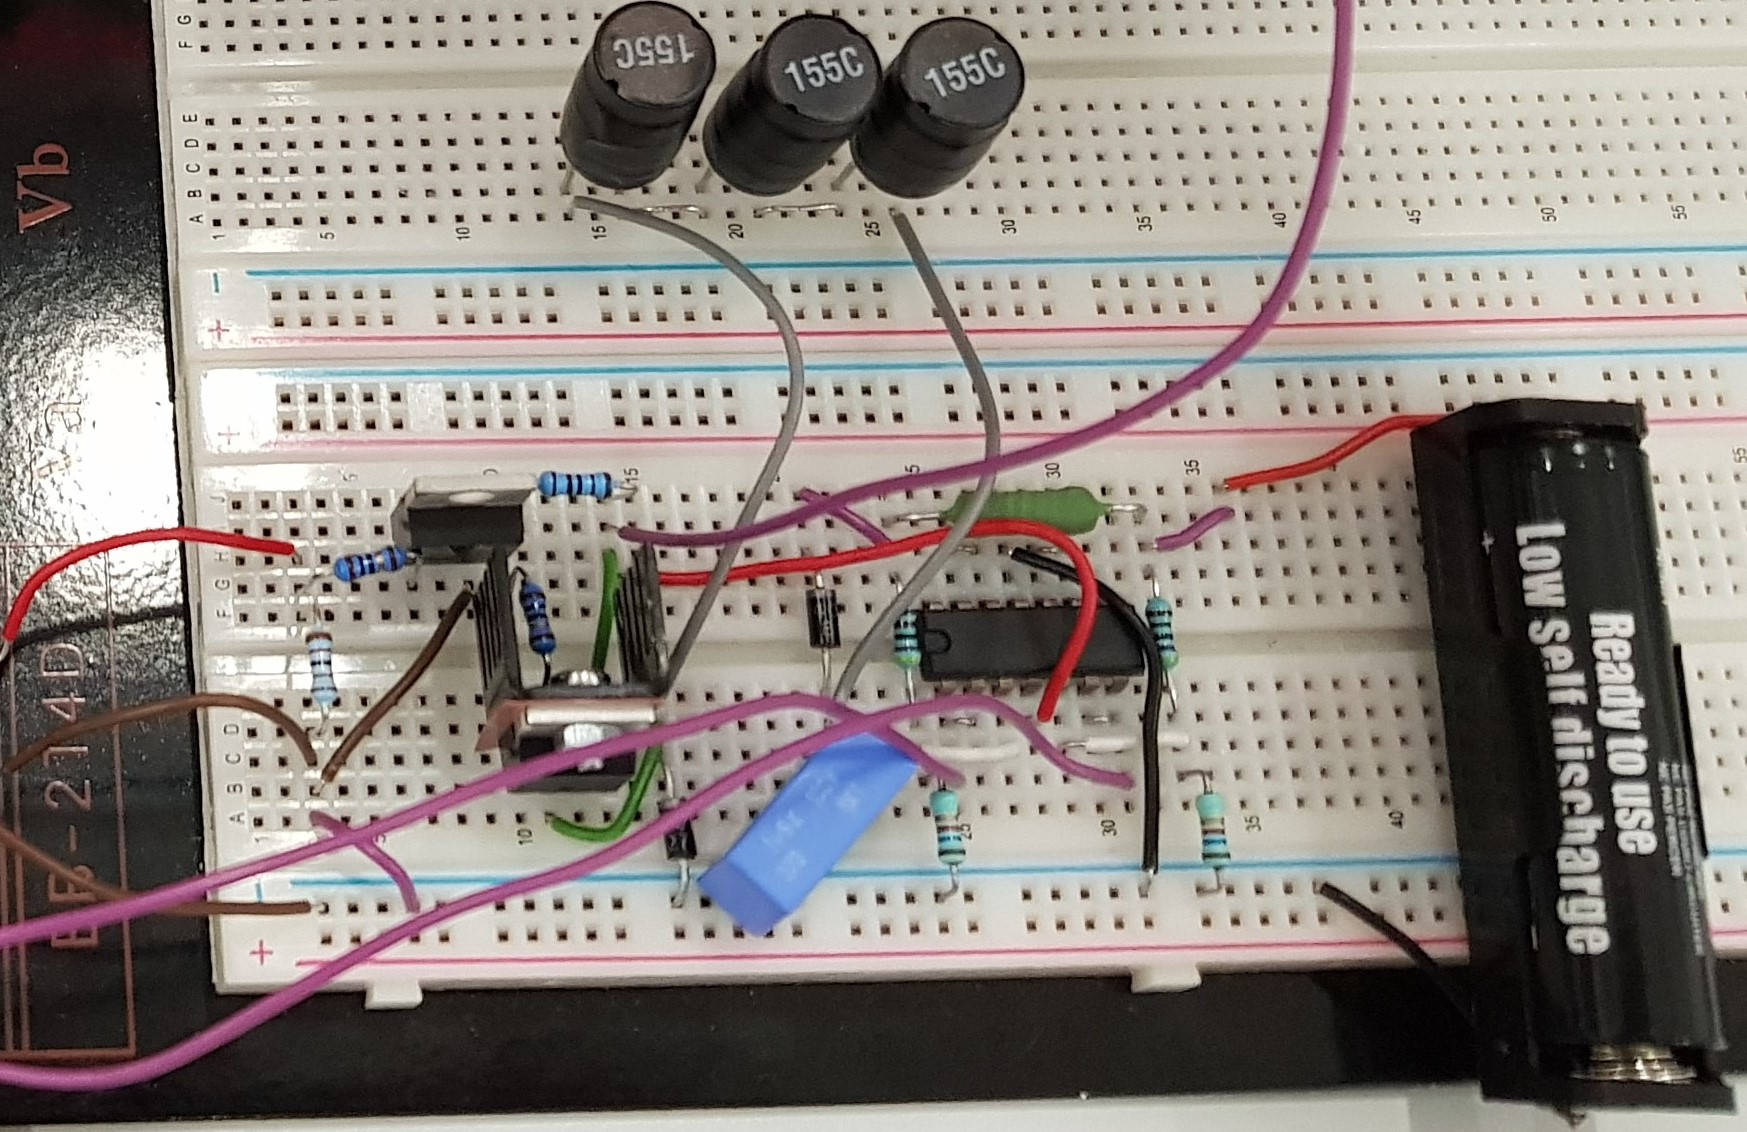
\includegraphics[width=1\textwidth]{figures/circuit/combined_triple_zoom.jpg}
     \caption{The designed charging circuit used for testing.}
     \label{fig:circuit:image}
\end{figure}
The circuit used for testing in this section is shown in \autoref{fig:circuit:image}.

\subsection{Measurements of the Circuit}
First the PWM module designed in \autoref{sec:pwm:module} is evaluated. A duty cycle of $50 \%$ is sent to the FPGA:
\begin{figure}[H]
    \centering
         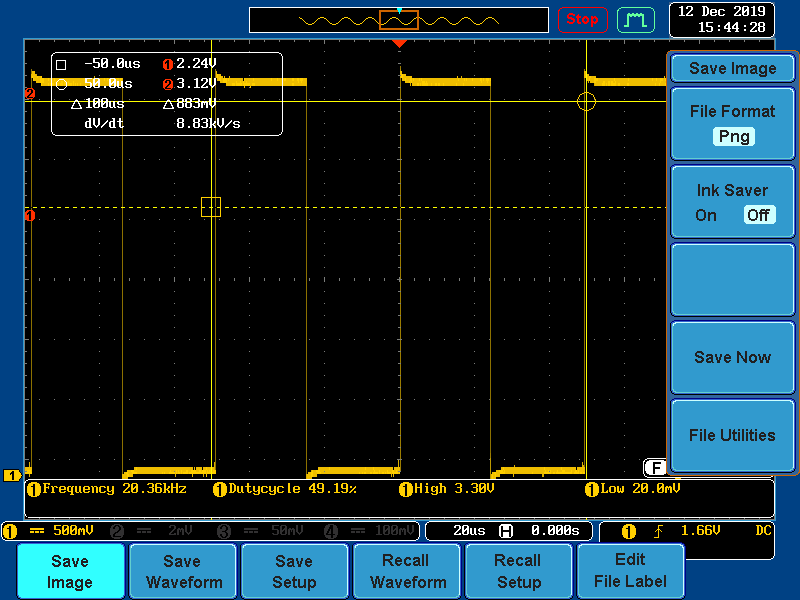
\includegraphics[width=0.7\textwidth]{figures/measurements/PWM_signal.PNG}
     \caption{The PWM signal generated by the FPGA.}
     \label{fig:pwm:measure}
\end{figure}
In \autoref{fig:pwm:measure} it is seen that the achieved frequency is approximately $20 [kHz]$ and the high and low voltage levels is approximately $0 [V]$ and $3.3 [V]$.\\
The PWM signal at the output of MOSFET $F_1$ is now measured to see if it correctly switches between $0 [V]$ and $12 [V]$ with a duty cycle of approximately $50 \%$ given the input PWM signal from the FPGA of approximately $50 \%$.
\begin{figure}[H]
    \centering
         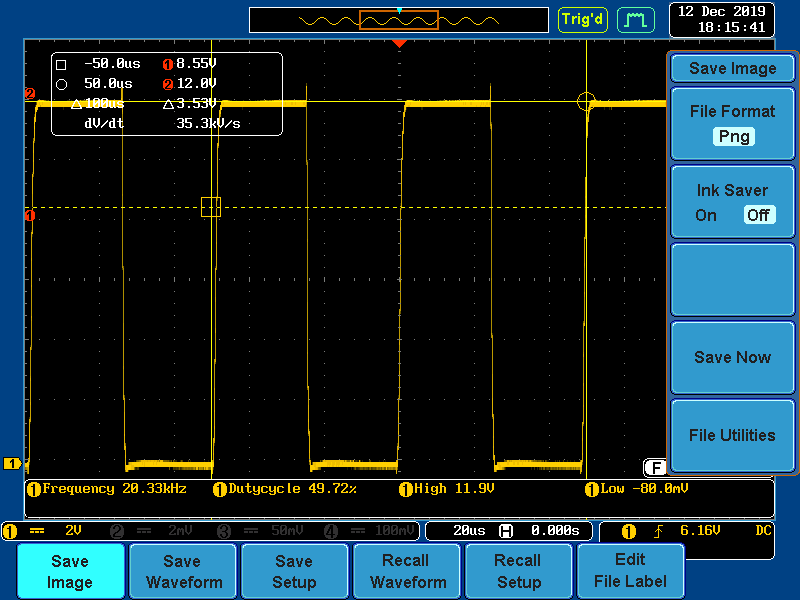
\includegraphics[width=0.7\textwidth]{figures/measurements/F1_mosfet.PNG}
     \caption{The output PWM signal of MOSFET $F_1$ switching between $0 [V]$ and $12 [V]$.}
     \label{fig:pwm:measure:F1}
\end{figure}
It is seen in \autoref{fig:pwm:measure:F1}, that the output of $F_1$ reaches the desired low of approximately $0 [V]$ and high level of approximately $12 [V]$ with the same duty cycle and frequency.\\
The output signal of the MOSFET $F_2$ is now measured to see if it correctly switch between $0 [V]$ and $12 [V]$.
\begin{figure}[H]
    \centering
         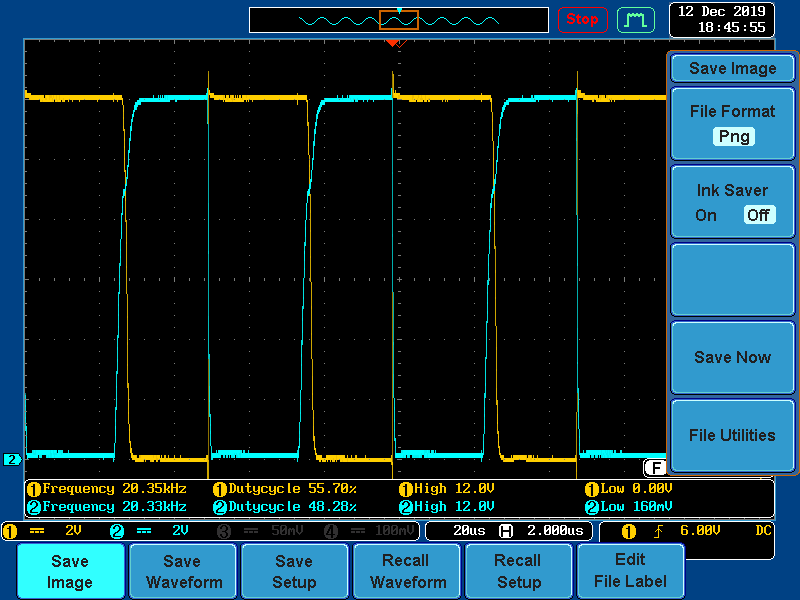
\includegraphics[width=0.7\textwidth]{figures/measurements/BOTH_mosfets.PNG}
     \caption{The output PWM signals of both MOSFETS $F_1$ and $F_2$. Channel 1 is output of $F_1$ and channel 2 is output of $F_2$.}
     \label{fig:pwm:measure:both}
\end{figure}
It can be seen in \autoref{fig:pwm:measure:both}, that the MOSFET $F_2$ switches between $0 [V]$ and $12 [V]$ as wanted at the same frequency and approximately same duty cycle.\\
The output of the buck converter is now measured. To do this a power resistor of size $30 [\Omega]$ is placed at the output of the buck converter, which acts as a load on the buck converter. The expected output is that the buck converter smooths the PWM signal with a ripple around the designed. The measurements is performed at duty cycles which creates an output of $1.5 [V]$, $3.0 [V]$, $4.5 [V]$ and $6.0 [V]$.
\begin{figure}[H]
    \centering
         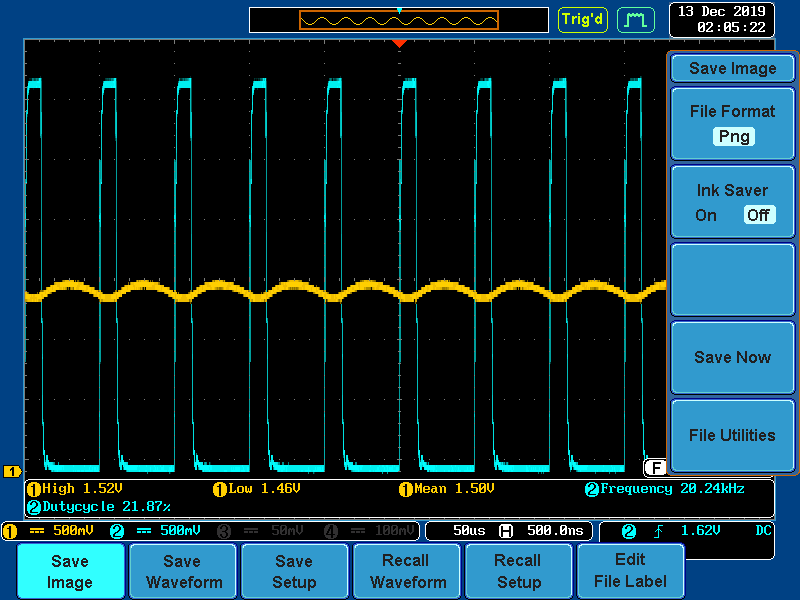
\includegraphics[width=0.7\textwidth]{figures/measurements/1_5_V_BOTH_PWRES.PNG}
     \caption{Channel 1 is the output of the buck converter with a load of $R = 33 [\Omega]$, channel 2 is the FPGA PWM input to the circuit. Target voltage is $1.5[V]$.}
     \label{fig:pwm:measure:buck_1_5}
\end{figure}
It can be seen in \autoref{fig:pwm:measure:buck_1_5}, that a duty cycle of $21.7 \%$ yields an output at the buck converter with an average of $1.5[V]$ and a ripple of $\Delta V_C = 0.040 V_{out}$.
\begin{figure}[H]
    \centering
         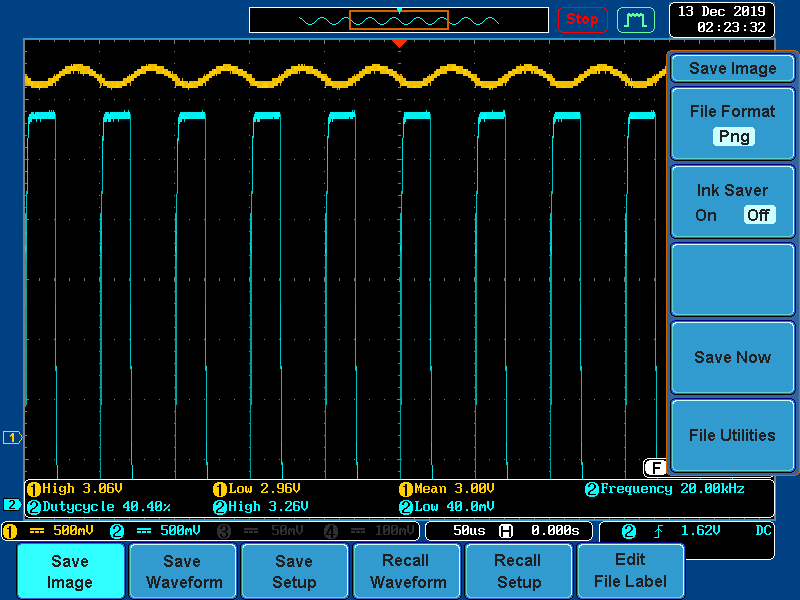
\includegraphics[width=0.7\textwidth]{figures/measurements/3_0_V_BOTH_PWRES.PNG}
     \caption{Channel 1 is the output of the buck converter with a load of $R = 33 [\Omega]$, channel 2 is the FPGA PWM input to the circuit. Target voltage is $3.0[V]$.}
     \label{fig:pwm:measure:buck_3_0}
\end{figure}
In \autoref{fig:pwm:measure:buck_3_0} it can be seen that a duty cycle of $40.4 \%$ yields an output at the buck converter with an average of $3.0 [V]$ with a ripple of $\Delta V_C = 0.033 V_{out}$.
\begin{figure}[H]
    \centering
         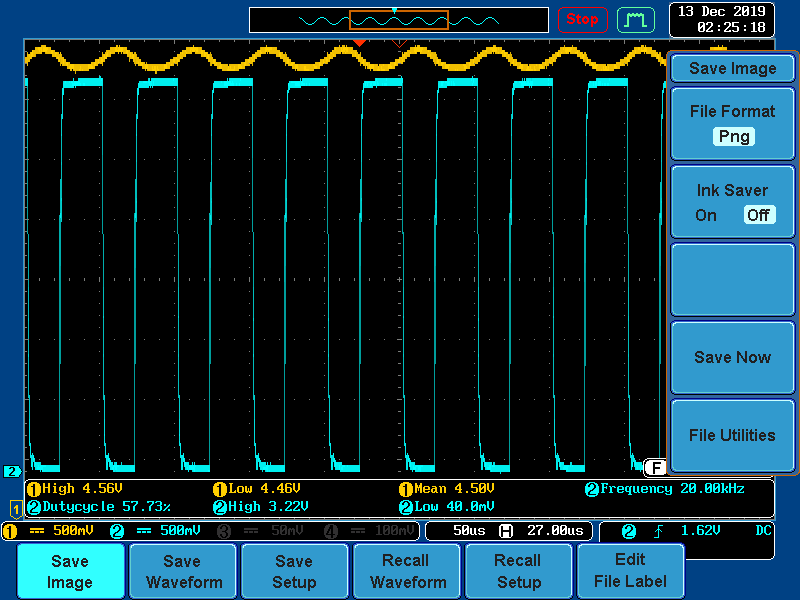
\includegraphics[width=0.7\textwidth]{figures/measurements/4_5_V_BOTH_PWRES.PNG}
     \caption{Channel 1 is the output of the buck converter with a load of $R = 33 [\Omega]$, channel 2 is the FPGA PWM input to the circuit. Target voltage is $4.5[V]$.}
     \label{fig:pwm:measure:buck_4_5}
\end{figure}
In \autoref{fig:pwm:measure:buck_4_5} it can be seen that a duty cycle of $57.73 \%$ yields an output at the buck converter with an average of $4.5 [V]$ with a ripple of $\Delta V_C = 0.022 V_{out}$.
\begin{figure}[H]
    \centering
         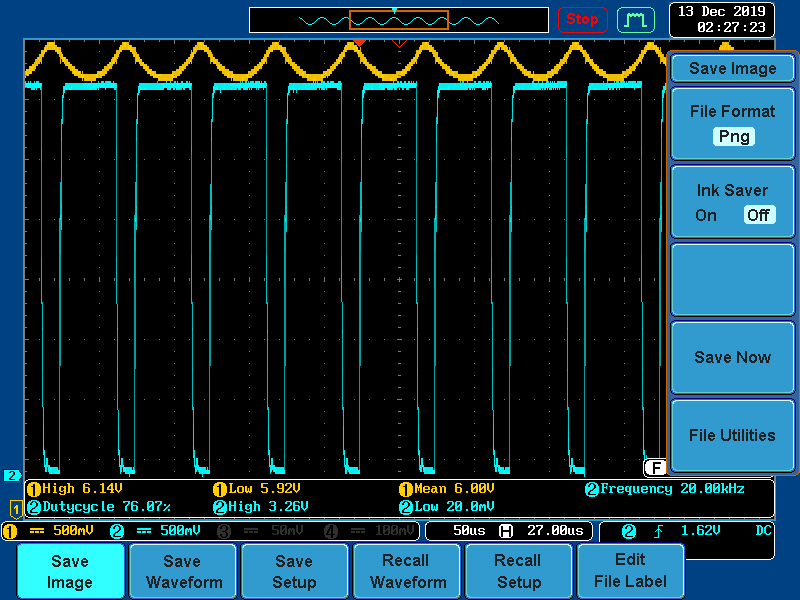
\includegraphics[width=0.7\textwidth]{figures/measurements/6_0_V_BOTH_PWRES.PNG}
     \caption{Channel 1 is the output of the buck converter with a load of $R = 33 [\Omega]$. Channel 2 is the FPGA PWM input to the circuit. Target voltage is $6.0[V]$.}
     \label{fig:pwm:measure:buck_6_0}
\end{figure}
In \autoref{fig:pwm:measure:buck_6_0} it can be seen that a duty cycle of $76.07 \%$ yields an output at the buck converter with an average of $6.0 [V]$ with a ripple of $\Delta V_C = 0.036 V_{out}$.\\
The ripple at the four voltage levels was at a maximum of $4 \%$ of the output voltage, which is acceptable. The battery is now placed at the output of the buck converter instead of the power resistor. 
%This might reduce the ripple of the buck converter output even further since the battery acts as a capacitor.
\begin{figure}[H]
    \centering
         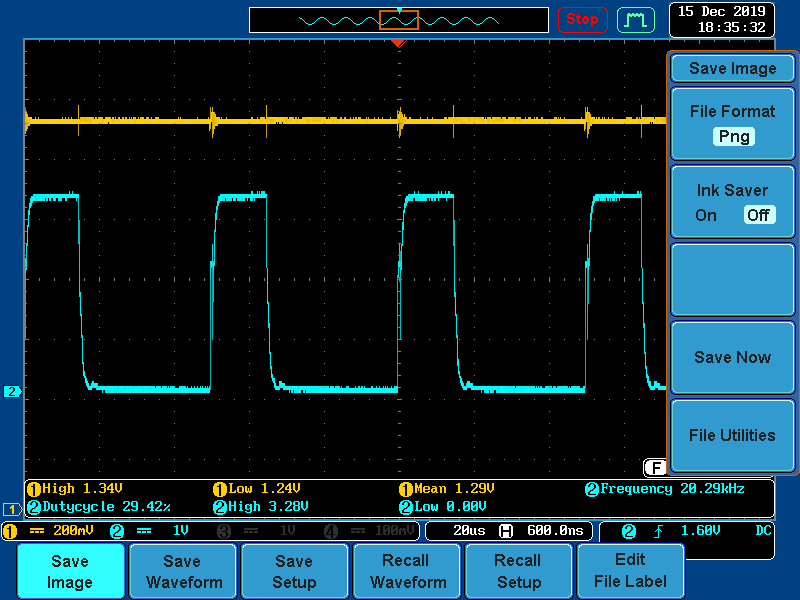
\includegraphics[width=0.7\textwidth]{figures/measurements/BATTERY_MEASURE.PNG}
     \caption{Channel 1 is the battery voltage, channel 2 is the FPGA PWM input to the circuit. Target current is $0.2[mA]$.}
     \label{fig:pwm:measure:battery}
\end{figure}
It is seen that the ripple is generally much lower in \autoref{fig:pwm:measure:battery} than the measurements with a load resistor, but there is some high frequent ripple present.

\subsection{Measurements of the Monitoring}
\begin{figure}[H]
    \centering
    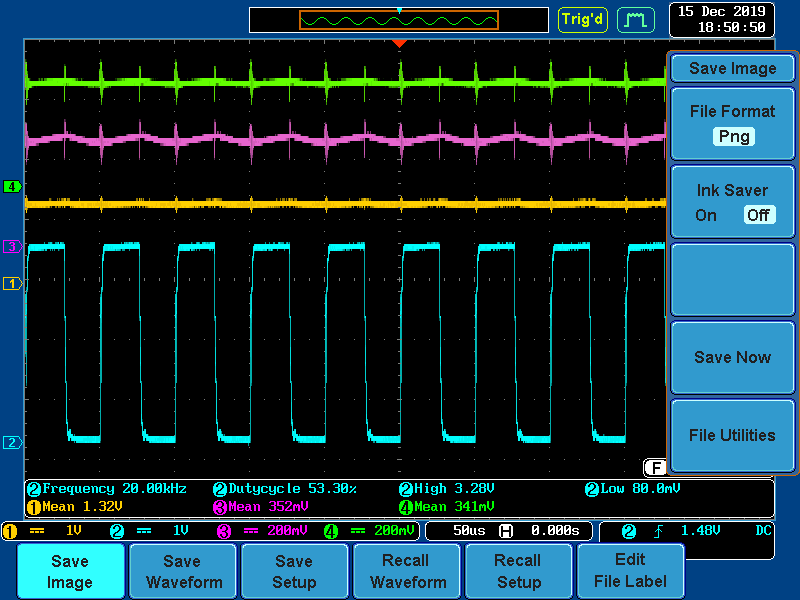
\includegraphics[width=0.7\textwidth]{figures/measurements/MONITOR.PNG}
    \caption{Channel 1 is the battery voltage, channel 2 is the FPGA PWM input to the circuit, channel 3 is the $V_{ADC1}$ signal and channel 4 is the $V_{ADC2}$ signal. Target current is $0.25[mA]$.}
    \label{fig:pwm:measure:battery}
\end{figure}
The actual value of $i_{charge}$, current drawn, by the battery was measured to be $i_{charge} = 254 [mA]$ using a digital multimeter. The two voltages for the ADCs were measured: $V_{ADC1} = 354 [mV]$ and $V_{ADC2} = 338 [mV]$, this yields the following calculation of battery voltage: $V_{Bat} = 3.9375\cdot V_{ADC2} = 1.33 [V]$, which is very close to the battery voltage (channel 1) in \autoref{fig:pwm:measure:battery}. The current $i_{charge}$ is calculated as $i_{charge} = 15.75 \left( V_{ADC1} - V_{ADC2} \right) = 252 [mA]$ which is very close to the one measured with the digital multimeter.

\subsection{The Combined System}
The combined system with the processing system and programmable logic combined with the designed electrical system is tested.
\begin{figure}[H]
    \centering
         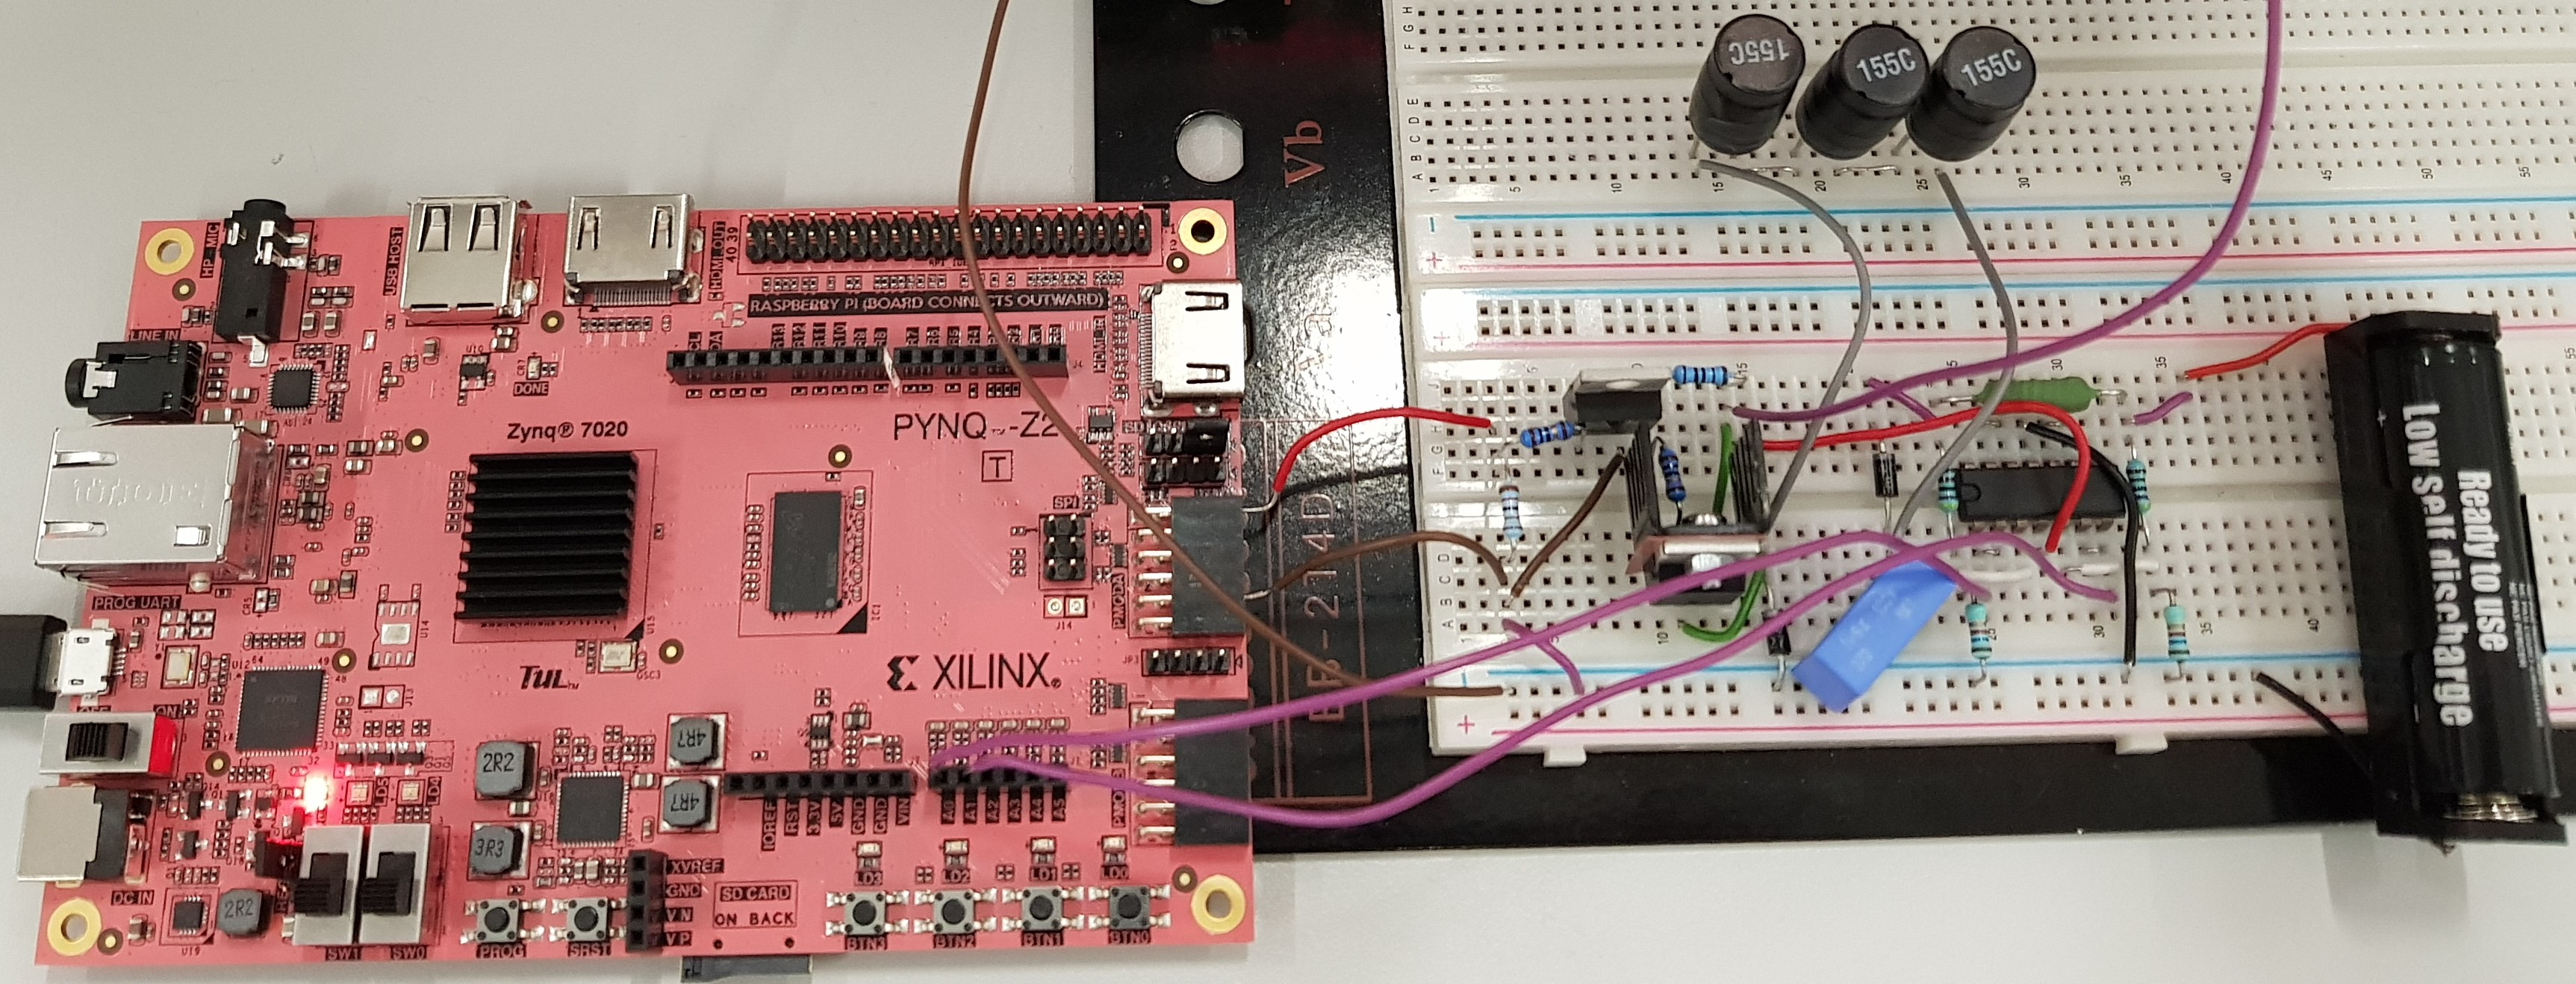
\includegraphics[width=1\textwidth]{figures/circuit/combined_triple.jpg}
     \caption{The combined system with the microprocessor, FPGA and charging circuit.}
     \label{fig:circuit:combined}
\end{figure}
The combined system is shown in \autoref{fig:circuit:combined}. The test is performed by first entering the following values:
\begin{enumerate}
    \item Nominal battery voltage: $V_{Bat(Nominal)} = 1.5 [V]$.
    \item Battery capacity: $Q = 2000 [mAh]$.
    \item Battery rate of charge: $C = 1$.
    \item Charging speed: $ k = 0.1$.
\end{enumerate}
By entering the above values the target current is $i_{target} = 0.2 [A]$. It is observed that the system balances the target current at around $i_{charge} = i_{target} = 0.2 [A]$.\\
A video of the test is uploaded to Youtube: \url{https://youtu.be/0lCbZjbHUG8}.

The combined solution is then tested if capable of charging a $3.0 [V]$ battery. The following values are entered in the terminal:
\begin{enumerate}
    \item Nominal battery voltage: $V_{Bat(Nominal)} = 3.0 [V]$.
    \item Battery capacity: $Q = 4000 [mAh]$.
    \item Battery rate of charge: $C = 1$.
    \item Charging speed: $ k = 0.1$.
\end{enumerate}
Using the above values the target current is  $i_{target} = 0.4 [A]$. It is observed that the system balances the target current at around $i_{charge} = i_{target} = 0.4 [A]$.\\
A video of the test is uploaded to Youtube: \url{https://youtu.be/0lCbZjbHUG8}.

Lastly, the combined solution is tested if capable of charging a $4.5 [V]$ battery. The following values are entered in the terminal:
\begin{enumerate}
    \item Nominal battery voltage: $V_{Bat(Nominal)} = 4.5 [V]$.
    \item Battery capacity: $Q = 6000 [mAh]$.
    \item Battery rate of charge: $C = 1$.
    \item Charging speed: $ k = 0.1$.
\end{enumerate}
Using the above values the target current is  $i_{target} = 0.6 [A]$. It is observed that the system balances the target current at around $i_{charge} = i_{target} = 0.6 [A]$.\\
A video of the test is uploaded to Youtube: \url{https://youtu.be/0lCbZjbHUG8}.

\end{document}